\documentclass{article}


% if you need to pass options to natbib, use, e.g.:
%     \PassOptionsToPackage{numbers, compress}{natbib}
% before loading neurips_2024

% ready for submission
% \usepackage{neurips_2024}

% to compile a preprint version, e.g., for submission to arXiv, add add the
% [preprint] option:
  % \usepackage[preprint]{neurips_2024}

% to compile a camera-ready version, add the [final] option, e.g.:
%     \usepackage[final]{neurips_2024}


% to avoid loading the natbib package, add option nonatbib:
  %  \usepackage[nonatbib]{neurips_2024}

\usepackage[preprint, nonatbib]{neurips_2024}

\usepackage{mymathstyle} % math macros

\usepackage[utf8]{inputenc} % allow utf-8 input
\usepackage[T1]{fontenc}    % use 8-bit T1 fonts
\usepackage{hyperref}       % hyperlinks
\usepackage{url}            % simple URL typesetting
\usepackage{booktabs}       % professional-quality tables
\usepackage{amsfonts}       % blackboard math symbols
\usepackage{nicefrac}       % compact symbols for 1/2, etc.
\usepackage{microtype}      % microtypography
\usepackage[dvipsnames]{xcolor}         % colors
\usepackage{cleveref}

\usepackage{paper_commands}

% region set up fixme and in-text annotations
\usepackage{pdfcomment}
% put draft in options if, otherwise remove
\usepackage[draft, noinline, margin, mode=multiuser, author=]{fixme}
\usepackage[us]{datetime}
\fxloadlayouts{pdfcnote}
\fxuseenvlayout{colorsig} % plain, signature, color, colorsig
\fxusetargetlayout{changebar} % plain, changebar, color, colorcb
\FXRegisterAuthor{aa}{anaa}{AA}
\FXRegisterAuthor{jl}{anjl}{JL}
\fxusetheme{colorsig}
\fxsetface{margin}{\scriptsize}
% endregion

% region hyperref and link color options
% \newcommand\myshade{100}
% \colorlet{mylinkcolor}{RubineRed}
% \colorlet{mycitecolor}{RoyalBlue}
% \colorlet{myurlcolor}{RoyalBlue}

\hypersetup{
  linkcolor  = RubineRed, %mylinkcolor!\myshade!black,
  citecolor  = RoyalBlue, %!\myshade!black,
  urlcolor   = RoyalBlue, %!\myshade!black,
  colorlinks = true,
}
% endregion

% region biblatex bibliography setup
\usepackage[backend=bibtex, style=authoryear-comp, date=year, maxbibnames=10, maxcitenames=2, url=false, uniquelist=false, isbn=false, doi=false, sortcites=false, dashed=false, natbib=true, backref=true]{biblatex}
\DefineBibliographyStrings{english}{%
  backrefpage = {cited on page},% originally "cited on page"
  backrefpages = {cited on pages},% originally "cited on pages"
}
\AtEveryBibitem{%
  \clearfield{volume}%
  \clearfield{number}
  \clearfield{pages}}
\DeclareFieldFormat{title}{\mkbibquote{#1}}
\addbibresource{references.bib}
% endregion

% NOTE: TEMPORARY TITLE
% what do we call this model? still Abstractor? Or AbstractTransformer?
% Or a name leaning towards the idea of it being more expressive and versatile through the mixture of specialized attention heads? (letting go of the "abstract" theme)
\title{More [versatile] [expressive] Inductive Biases in Transformer Architectures through Mixtures of Specialized Attention Heads}

% The \author macro works with any number of authors. There are two commands
% used to separate the names and addresses of multiple authors: \And and \AND.
%
% Using \And between authors leaves it to LaTeX to determine where to break the
% lines. Using \AND forces a line break at that point. So, if LaTeX puts 3 of 4
% authors names on the first line, and the last on the second line, try using
% \AND instead of \And before the third author name.


\author{%
  Awni Altabaa\\ % \thanks{Use footnote for providing further information
    % about author (webpage, alternative address)---\emph{not} for acknowledging
    % funding agencies.} \\
  Department of Statistics \& Data Science\\
  Yale University\\
  \texttt{awni.altabaa@yale.edu} \\
  \And
  John Lafferty \\
  Department of Statistics \& Data Science \\
  Yale University \\
  \texttt{john.lafferty@yale.edu}
  % should we include WTI/FDS affiliation for John
}

\begin{document}

\maketitle


\begin{abstract}
  The Transformer architecture processes sequences by implementing a form of neural message-passing that consists of iterative information retrieval (attention), followed by local processing (position-wise MLP).
  We argue that for such a procedure, two types of contextual information are crucial: 1) object-level features of attended objects, and 2) the \textit{relations} between these objects and the receiver.
  Standard attention naturally captures the former, but does not explicitly support the latter.
  In this paper, we present an extension of Transformers where multi-head attention now consists of two distinct types of ``attention heads,'' each handling routing information of a different type. The first is the standard attention mechanism of Transformers which captures object-level features, while the second is a novel attention mechanism we propose that captures relational features.
  The two types of attention heads each possess different inductive biases, giving the resulting architecture greater efficiency and versatility.
  Empirical evaluation across a range of tasks, including visual relational reasoning, mathematical problem solving, and language modeling, demonstrates the promise of this approach.
\end{abstract}

\tableofcontents

\newpage

\section{Introduction}\label{sec:intro}

\aawarning{TODO---update abstract...}

A central goal of machine learning research is to develop unified architectures capable of learning and reasoning across a wide range of tasks and data modalities. However, there is a tension between the goal of creating a general architecture and the need to support inductive biases that are beneficial for certain types of tasks~\citep{wolpert1995no,baxter2000model}. With a finite training set and multiple possible solutions for empirical risk minimization, inductive biases guide the learning algorithm to prioritize solutions with specific properties, thereby enabling greater data efficiency and improved generalization to new inputs. A tantalizing hypothesis is that human and animal intelligence can be explained by a small set of fundamental principles~\citep{marcus2003algebraic}. In the context of machine intelligence, our goal is to uncover a complete set of fundamental inductive biases with broad applicability to real-world tasks that enable robust, flexible, and data-efficient learning.

Such a unified architecture must be capable of handling general inputs of various modalities and must possess computational mechanisms for routing and processing both the attributes of objects in the input and the relations between them. In analogy to neural systems in the brain~\citep{newman1997neural}, we refer to the former as \textit{sensory} information and the latter as \textit{relational} information.

The Transformer architecture~\citep{vaswani2017attention} provides a promising candidate for the basis of a versatile general-purpose architecture for machine learning. By operating over sets or sequences of objects, Transformers are able to support highly-general inputs and outputs. More importantly, neural attention provides an effective computational mechanism for routing sensory information between different elements in the input, enabling iterative contextual processing. This has lead to remarkable empirical success across several domains, including language~\citep{kaplan2020scalinglawsneurallanguage} and visual processing~\citep{dosovitskiyImageWorth16x162020}.

Yet, recent work on relational learning has shown that Transformers struggle to efficiently learn tasks involving relational reasoning, prompting several proposals for neural architectures that incorporate inductive biases for relational learning~\citep{santoroSimpleNeuralNetwork2017,santoroRelationalRecurrentNeural2018,shanahanExplicitlyRelationalNeurala,webbEmergentSymbolsBinding2021,webbRelationalBottleneckInductive2024,kergNeuralArchitectureInductive2022,altabaa2024abstractors,altabaaLearningHierarchicalRelational2024}. Relational reasoning is an essential component of general intelligence, making the lack of support for efficient and robust relational learning a fundamental limitation of the Transformer framework. The ultimate power of relational reasoning lies in its capacity to to generate inferences and generalizations in systematic and novel ways, which, in the limit, can lead to universal inductive generalization from a small set of observations to a potential infinite set of novel instances~\citep{goyal2022inductive}.

In this paper, we posit the following explanation for the Transformer's limited abilities in relational learning: while neural attention provides a powerful mechanism for routing \textit{sensory} information between objects in the input, the Transformer lacks an explicit computational mechanism for routing and processing \textit{relational} information between objects. Thus, we argue that standard Transformers possess an incomplete set of inductive biases, notably lacking inductive biases for relational learning. The goal of this paper is to propose an extension of the Transformer framework which enables explicit routing and processing of both sensory and relational information.

To understand our proposed method at a high-level, it can be useful to view standard Transformers as an instantiation of a broader neural message-passing computational paradigm that consists of iterative information retrieval followed by local processing. In its general form, a collection of objects $x_1,\ldots, x_n$ are processed via an iterative application of
\begin{equation}\label{eq:intro_message_passing}
  \begin{split}
    x_i &\gets \mathrm{Aggregate}\bigparen{x_i, \set{m_{j \to i}}_{j=1}^{n}}, \\
    x_i &\gets \mathrm{Process}(x_i).
  \end{split}
\end{equation}
In the case of Transformers, the self-attention mechanism can be seen as sending messages from object $j$ to object $i$ that are encodings of the sender's \textit{sensory} features, with the message from sender $j$ to receiver $i$ given by $m_{j \to i} = \phi_v(x_j)$. These messages are then aggregated according to some selection criterion based on the receiver's features, typically determined by softmax attention scores.

To enable explicit relational representation learning, we propose a novel attention mechanism that attends over and routes the relational information between objects in the input. In \textit{relational attention}, the message from the sender object to the receiver object is a set of relations between them, which can be expressed as $m_{j \to i} = r(x_i, x_j)$. Here, the relation $r(\cdot, \cdot)$ models a series of comparisons between objects across different feature dimensions dimensions via inner products of feature maps. We combine this with the standard attention mechanism of of Transformers yielding a variant of multi-head attention for processing both sensory and relational information. This \textit{Dual Attention} architecture disentangles the two types of information in the aggregation phase of attention, while integrating them during the information processing stage.

The contributions in this paper are summarized as follows:
\begin{enumerate}
  \item We introduce a new \textit{relational attention} mechanism that disentangles sensory information from relational information. While standard self-attention models retrieval of sensory information, relational attention models retrieval of relational information.
  \item We introduce an extension of the Transformer architecture that integrates sensory and relational information through \textit{Dual Attention}---a form of multi-head attention with two distinct types of attention heads. Standard self-attention heads encode sensory information, while relational attention heads encode relational information.
  \item We carry out a thorough and diverse set of experiments, showing that the \textit{Dual Attention Transformer} outperforms standard Transformers in terms of data efficiency across a range of tasks, suggesting that relational inductive biases are an important component of the general machine intelligence and learning systems we seek.
\end{enumerate}

\begin{figure}[t]
  \centering
  \begin{subfigure}[t]{0.415384615\textwidth} % 0.9 * 3 / 6.5
    \centering
    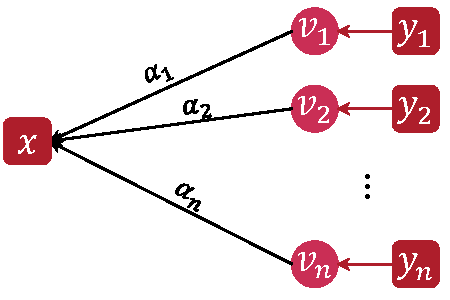
\includegraphics[width=\textwidth]{figs/sensory_retrieval.pdf} % size: 3 x 2 in
    \caption{$\Attn(x, \ys)$}%: Retrieval of sensory information by standard attention.}
  \end{subfigure}
  \qquad
  \begin{subfigure}[t]{0.484615385\textwidth} % 0.9 * 3.5 / 6.5
    \centering
    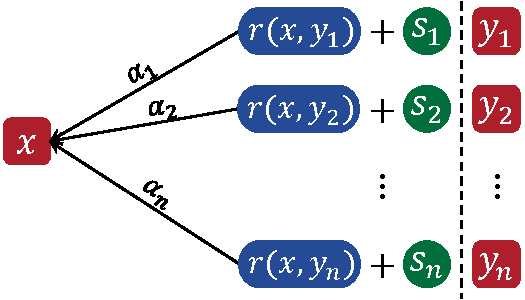
\includegraphics[width=\textwidth]{figs/relational_retrieval.pdf} % size 3.5 x 2 in
    \caption{$\RelAttn(x, \ys)$}%: Retrieval of relational information by relational attention.}
  \end{subfigure}
  % 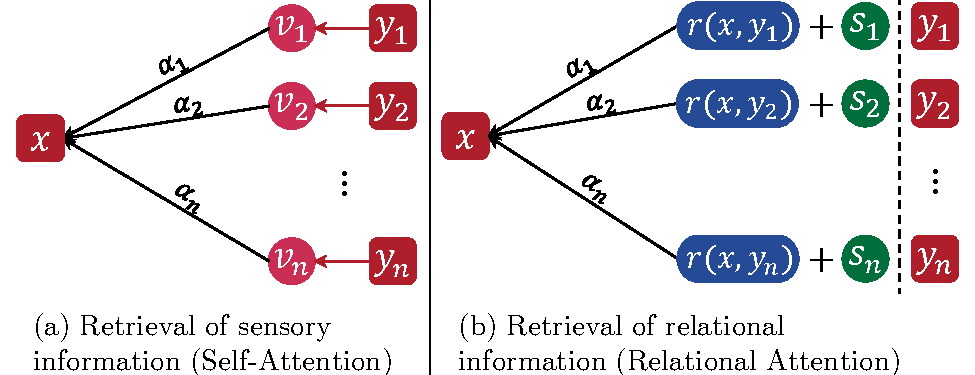
\includegraphics[width=0.8\textwidth]{figs/attn_fig_combined_noqeuerykey.pdf}
  \caption{Standard self-attention retrieves sensory information $v_i$ about the attributes of individual objects while \textit{relational attention} retrieves relational information $r(x, y_i)$ about the relationship between the objects in the context and the receiver.
  Each relation is tagged with a symbol $s_i$ which acts as an abstract variable identifying the sender.
  In both cases, information is aggregated according to the attention scores $\alpha_i$, which are computed by a softmax over inner products of queries and keys.
  }\label{fig:selfattn_relattn}
  \vskip-7pt
\end{figure}

\aawarning{TODO---expand on experiments? mention type of experiments we ran and their scale? that we explored scaling laws, etc.}

\section{Abstract Attention: Mixture of specialized attention heads}
\aanote{is ``abstract attention'' a good name?}

\begin{enumerate}
  \item The core component of standard Transformers is self-attention (and cross-attention, in encoder-decoder Transformers). Intuitively, what self-attention does is to route information between elements in the sequence. A Transformer block is simply composing self-attention with a feedforward network to perform independent element-wise processing (modulo technicalities such as layer normalization, residual connections, etc).
  \item Simply stacking these simple blocks leads to remarkable scalability in various domains, including language, vision, etc.
  \item At its core, all self-attention does is route information. By contrast, relational cross-attention is focused on extracting \textit{relational information}. Both aspects are crucial for general sequence-modeling.
  \item We hypothesize that imbuing a Transformer with additional more specialize ``attention heads'' will enable the model to learn more robust, generalizable representations in a more sample-efficient manner.
  \item The intuitive reason for this hypothesis is that self-attention is a single type of computation: it can only select and retrieve information. Adding more and more self-attention heads will saturate: the mode already did all it can with this type of computation. If we instead add a different kind of attention head (i.e., RCA) the model will now have a different kind of computation available to it, which will be useful in new and different ways. By having both kinds of computation available to the model, it can learn to use both and select between them depending on the current context/etc. [this is the basic idea, but TO-DO: revise sentence and make it flow better. improve argument. etc.]
\end{enumerate}

\section{Disentangling Attention over Sensory and Relational Information}

\subsection{Standard Attention: Attention over Sensory Information}

The attention mechanism of standard Transformers can be understood as a form of neural message-passing that performs selective information retrieval. Each object emits a query which is compared against the keys of each object in its context via an inner product. A ``match'' occurs when the inner product is large, causing the features of the attended object to be retrieved and added to the residual stream of the ``receiver''. Formally, self-attention takes the form\aanote{add somehwere, perhaps as footnote: throughout the paper, we will use the generic term ``object'' to refer to elements of the sequence/set input (e.g., tokens in the context of text or patches of an image in the context of vision, etc.)}
\begin{equation}\label{eq:self_attn}
  \begin{split}
    \Attn(x, \ys) &= \sum_{i=1}^{n} \alpha_i(x, \y) \phi_v(y_i) \\
    \alpha(x, \y) &= \Softmax\bigparen{\bra{\iprod{\phi_q(x)}{\phi_k(y_i)}}_{i=1}^{n}},
  \end{split}
\end{equation}
where $\phi_q,\phi_k$ are the query/key mappings controlling the ``selection criterion'' and $\phi_v$ is the value mapping controlling what information the attended objects ``send''. $\phi_q, \phi_k, \phi_v$ are typically implemented as learnable linear maps. The attention scores $\alpha(x, \y) \in \Delta^n$ retrieve a convex combination of the values.

The information being retrieved here is ``sensory'' information---that is, the object-level features of the selected objects. There is no explicit retrieval of a representation of the relation between the sender and the receiver. The attention scores $\alpha_i(x, \y)$ can perhaps be thought of as (normalized) relations between objects, but these are merely computed as an intermediate step in an information-retrieval operation, and are ultimately entangled with the object-level of the sender\footnote{In principle, it is also possible that the MLP compute a relation between the sender and receiver in the ``local processing'' step by separating out their representations and computing a comparison. However, this is difficult to do since the representations of the objects will be additively mixed, and there is no inductive bias pressuring the computed function to be a relation.}. This makes learning relational representations in standard Transformers inefficient.

\subsection{Disentangled Relational Attention: Attention over Relational Information}

We propose a type of ``attention head'' with a relational inductive bias. Under the message-passing view (\Cref{eq:intro_message_passing}), the message from one object to another encodes the relation between the sender and the receiver. We call this operation (Disentangled) Relational Attention.

At a high-level, this operation begins in the same way as the standard attention mechanism, with each object emitting a query and a key, which are compared via an inner product. When the inner product is high, an object is ``selected''. But, now rather than retrieving the features of the selected object, what is retrieved is the \textit{relation} between the two objects. In addition, we must send an identifier that signifies to the receiver ``who the relation is with''. Mathematically, this operation is defined as follows.
\begin{equation}\label{eq:rel_attn}
  \begin{split}
    \RelAttn(x, \ys) &= \sum_{i=1}^{n} \alpha_i(x, \y) \bigparen{W_r \, r(x, y_i) + W_s \, s_i}, \\
    \alpha(x, \y) &= \Softmax\bigparen{\bra{\iprod{\phi_q^{\attn}(x)}{\phi_k^{\attn}(y_i)}}_{i=1}^{n}}, \\
    r(x, y) &= \bigparen{\iprod{\phi_{q,1}^{\rel}(x)}{\phi_{k,1}^{\rel}(y)}, \ldots, \iprod{\phi_{q, d_r}^{\rel}(x)}{\phi_{k, d_r}^{\rel}(y)}} \in \reals^{d_r}, \\
    (s_1, \ldots, s_n) &= \mathrm{SymbolAssignment}(\ys)
  \end{split}
\end{equation}

Thus, relational attention between the object $x$ and the context $\y = \ys$ retrieves a convex combination of $x$'s relations with each object in the context $r(x, y_i)$, each marked with a ``symbol'' $s_i$ which identifies the sender. We will expand on the role and implementation of the symbols in the next subsection. Here, $\phi_q^{\attn}, \phi_k^{\attn}$ are learned feature maps which control the selection criterion for which object(s) in the context to attend to. Another set of query/key feature maps, $\phi_{q,i}^{\rel}, \phi_{k,i}^{\rel}, i \in [d_r]$, are learned to represent the relation between the sender and the relation. Each inner product $\iprod{\phi_q^{\rel}(x)}{\phi_k^{\rel}(y)}$ can be thought of as a comparison of the two objects' features under a particular filter---a `relation'. The $d_r$ (pairs) of feature maps produce a $d_r$-dimensional relation vector.

In some tasks, a good inductive bias on the relations is \textit{symmetry}: the relation between $x$ and $y$ is the same as the relation between $y$ and $x$. This can be achieved by using the same feature filter for the query and key map (i.e., $\phi_q^{\rel} = \phi_k^{\rel}$). This imbues the relations with added structure, making them positive semi-definite kernels which define a pseudometric on the object space and a corresponding geometry. We explore this and expand on this discussion in our experiments.

\subsection{Symbol Assignment Mechanisms}

For the purposes of processing relations, all the receiver needs to know is: 1) the relation between itself and the objects in its context, and 2) the identity of the object corresponding to each relation. The role of the ``symbols'' in (disentangled) relational attention is to ``tag'' the relations with the identities of the objects with which the relations are with. Without this, the result of relational attention will be an aggregated representation of the relations between the receiver and the selected object(s), without encoding ``who the relations are with''.

A symbol ``identifies'' or ``refers to'' an object, but, importantly, without fully encoding the features of the object. The second point is what makes relational attention (\Cref{eq:rel_attn}) ``disentangled'' from sensory or object-level features. The sensory features of individual objects are high-dimensional and have a lot of variability. By contrast, relational information is low-dimensional and more ``abstract''. If sensory object-level features are mixed with relational information, they would overwhelm the relational information, preventing abstraction and generalization. Instead, symbols act as abstract references to objects, perhaps thought of as a connectionist analogue of pointers in traditional symbolic architectures.

Here, the ``identity'' of an object may mean different things in different situations. For us, identity may be encoded by 1) position, 2) relative position, or 3) an equivalence class over features. We consider three different symbol assignment mechanisms corresponding to each.

\textbf{Positional Symbols.} In some applications, it is sufficient to identify objects through their position in the input sequence. We maintain a library of symbols $\Slib = (s_1, \ldots, s_{\mathtt{max\_len}}) \in \reals^{\mathtt{max\_len} \times d_{\mathrm{model}}}$ and assign $s_i$ to the $i$-th object in the sequence. These are essentially learned positional embeddings.

\textbf{Position-Relative Symbols.} Sometimes, the more relevant identifier is \textit{relative} position with respect to the receiver, rather than absolute position. This can be implemented with position-relative embeddings. We learn a symbol library $\Slib = (s_{-\Delta}, \ldots, s_{-1}, s_0, s_1, \ldots, s_{\Delta}) \in \reals^{(2 \Delta + 1) \times d_{\mathrm{model}}}$, and relational attention becomes $x_i' \gets \sum_{j} \alpha_{ij} (W_r \, r(x_i, x_j) + W_s \, (s_{j-i}))$, with ``$m_{j \to i} = (r(x_i, x_j), s_{j-i})$.

\textbf{Symbolic Attention.} In certain domains, some information about the objects' features is necessary for ``identifying'' it for the purposes of relational processing. Yet, recall that we would like to avoid sending a full encoding of object-level features in order to maintain a relational inductive bias and ability for \aanote*{or ``generalization''}{abstraction} across relations. In ``symbolic attention'', we learn a \textit{finite} set of symbol vectors, $\Slib = (s_1, \ldots, s_{n_s}) \in \reals^{n_s \times d_{\mathrm{model}}}$, and a matching set of ``feature templates'' $\Flib = (f_1, \ldots, f_{n_s})$. We retrieve a symbol for each object by attention operation which matches the input vectors 
$x_i$ against the feature templates $f_j$, and retrieves symbols $s_j$.
\begin{equation}
  \SymbolicAttn(\x) = \Softmax\bigparen{(\x \, W_q)\, \Flib^\top} \Slib.
\end{equation}
Here, $\Slib, \Flib, W_q$ are learned parameters. This can be thought of as implementing soft differentiable ``equivalence classes'' over feature embeddings. Crucially, the number of symbols (i.e., ``feature equivalence classes'') is finite, which enables relational attention to still produce a relation-centric representation while tagging the relations with the necessary identifier. Our implementation allows for a multi-head variant of this operation.

In our experiments, we find that different symbol assignment mechanisms are more effective in different domains.

\aanote{do we nice to cite ourselves here?}

\aanote{Symbols as ``codes'' that identify objects without encoding their features.}

\subsection{Approximation theory: What Class of Functions can Relational Attention Compute?}

The following theorem says that an Disentangled Relational Attention can approximate any function on $\calX \times \calY^n$ which 1) selects an element in $\ys$, then 2) computes a relation with it. Both the selection criterion and the relation function are arbitrary, and the selection criterion is query-dependent.
\begin{theorem}[Informal]
  Let $\mathrm{Select}: \calX \times \calY^n \to \calY$ be an arbitrary ``preference selection'' function, which selects an element among $\ys$ based on a query-dependent partial order relation $\{\preceq_x\}_{x \in \calX}$. Let $r: \calX \times \calY \to \reals^{d_r}$ be an arbitrary continuous relation function on $\calX \times \calY$. For any such $\mathrm{Select}$ and $r$, there exists an Disentangled Relational Attention module which approximates the function $r(x, \mathrm{Select}(x, \y))$ to arbitrary precision.
\end{theorem}

\subsection{Technical Details: Multi-Head Variant, Causality, \& Positional Encoding}
\aawarning{TODO}
\aanote{This section can be moved to appendix and referenced from main text?}

\textbf{Multi-head variant.}

\textbf{Causality}

\textbf{Positional Encoding.} compatbility with different positional encodings: RoPE, relative-positional encoding, etc (incorporated in $\alpha$)


\section{Abstract Attention: Mixture of specialized attention heads}
\aanote{is ``abstract attention'' a good name?}

\begin{enumerate}
  \item The core component of standard Transformers is self-attention (and cross-attention, in encoder-decoder Transformers). Intuitively, what self-attention does is to route information between elements in the sequence. A Transformer block is simply composing self-attention with a feedforward network to perform independent element-wise processing (modulo technicalities such as layer normalization, residual connections, etc).
  \item Simply stacking these simple blocks leads to remarkable scalability in various domains, including language, vision, etc.
  \item At its core, all self-attention does is route information. By contrast, relational cross-attention is focused on extracting \textit{relational information}. Both aspects are crucial for general sequence-modeling.
  \item We hypothesize that imbuing a Transformer with additional more specialize ``attention heads'' will enable the model to learn more robust, generalizable representations in a more sample-efficient manner.
  \item The intuitive reason for this hypothesis is that self-attention is a single type of computation: it can only select and retrieve information. Adding more and more self-attention heads will saturate: the mode already did all it can with this type of computation. If we instead add a different kind of attention head (i.e., RCA) the model will now have a different kind of computation available to it, which will be useful in new and different ways. By having both kinds of computation available to the model, it can learn to use both and select between them depending on the current context/etc. [this is the basic idea, but TO-DO: revise sentence and make it flow better. improve argument. etc.]
\end{enumerate}

\section{Orthrus: The Dual-Head Transformer Architecture}

\subsection{Dual-Head Attention}

One of the keys to the success of the Transformer architecture is the use of so-called ``multi-head'' attention. This involves learning and computing multiple attention operations in parallel at each layer and concatenating the output. This enables learning multiple useful criteria for routing information between objects. However, all these attention heads share the same inductive bias, focusing on ``sensory'' information about individual objects. Intuitively, this leads to ``diminishing returns'' where adding more heads does not result in improved performance since all heads perform the same type of computation. In particular, a key type of inductive bias that a standard Transformer lacks is an inductive bias for processing \textit{relational} information between objects.

We posit that ``sensory'' and ``relational'' information are the two primary types of information that are of relevance when processing sequences or collections of objects. This idea has some support \aanote*{motivations/support/roots... The congitive neuroscience literature contains work in support of this hypothesis regarding how the human mind works.}{support} in cognitive (neuro)science~\citep{citation}. In this paper, we explore the effects of augmenting a Transformer with a specialized attention operation with relational inductive biases. We propose a type of ``multi-head'' attention with two distinct types attention heads: standard self-attention, and (disentangled) relational attention. Our hypothesis is that by having both kinds of computations available to the model, it can learn to use both and select between them depending on the current task/context/etc.

\Cref{alg:dual_head_attn} describes the proposed operation. The number of self-attention heads $n_h^{sa}$ and number of relational attention heads $n_h^{ra}$ are hyperparameters. The self-attention heads attend to and retrieve ``sensory'' information on the features of individual objects in the context while the relational attention heads attend to and retrieve ``relational'' information. The $n_h = n_h^{sa} + n_h^{ra}$ heads are then concated to produce the output. The result is a representation of contextual information with disentangled sensory and relational components.

We note that a symmetry inductive bias can be injected into the relations $\bm{r}_{ij}$ by imposing that $W_{q}^{\rel} = W_k^{\rel}$. We refer the reader to~\Cref{sec:appendix_implementation} for further discussion and implementation details.

\aanote{should we call it ``dual-head'' or ``dual head-type'' or ``dual-type''}

\begin{algorithm}[ht!]
	\caption{Dual-Head Attention}\label{alg:dual_head_attn}
	\SetKwInput{Hyperparameters}{Hyperparameters}
	\SetKwInput{Input}{Input}
	\SetKwInOut{Output}{Output}
    \Hyperparameters{$n_h^{sa}, n_h^{ra}$, symbol assignment mechanism, (optional: \texttt{symmetric\_RA = False}, $d_r = n_h^{ra}$, ...)}
	\Input{$\x = (x_1, \ldots, x_n) \in \reals^{n \times d}$ }

    \vspace{1em}

    \texttt{Compute self-attention heads}
    \begin{align*}
        \bm{\alpha}^{(h)} &\gets \Softmax\bigparen{{(W_q^h\, \x)} {(W_k^h\, \x)}^\intercal}, \qquad && h \in [n_h^{sa}] \\
        e_i^{(h)} &\gets \sum_{j} \alpha_{ij}^{(h)} W_v\, x_j, \qquad && i \in [n]\\
        e_i &\gets W_o \, \concat(e_i^{(1)}, \ldots, e_i^{(n_h^{sa})}), && i \in [n]
    \end{align*}

    \texttt{Assign symbols:} $\s = (s_1, \ldots, s_n) \gets \SymbolRetriever(\x)$

    \texttt{Compute relational attention heads}
    \begin{align*}
        \bm{\alpha}^{(h)} &\gets \Softmax\bigparen{{(W_q^{\attn,h}\, \x)} {(W_k^{\attn,h}\, \x)}^\intercal}, \qquad && h \in [n_h^{ra}] \\
        \bm{r}_{ij} &\gets \bigparen{\iiprod{W_q^{\rel, \ell} x_i}{W_k^{\rel,\ell} x_j}}_{\ell \in [d_r]} \qquad && i,j \in [n] \\
        a_i^{(h)} &\gets \sum_{j} \alpha_{ij}^{(h)} \bigparen{W_r^h \, \bm{r}_{ij} + W_s^{h}\, s_j}, \qquad && i \in [n],\, h \in [n_h^{ra}]\\
        a_i &\gets W_o \, \concat(a_i^{(1)}, \ldots, a_i^{(n_h^{ra})}), && i \in [n]
    \end{align*}

    \Output{$\bigparen{\concat(e_i, a_i)}_{i=1}^{n}$}

\end{algorithm}

\textbf{Attention Masks \& Causality.} Any type of attention mask (e.g., causal mask for autoregressive language modeling) can be implemented in relational attention in the same way as for standard self-attention (i.e., mask is added to $\alpha_{ij}^h$ pre-softmax).

\textbf{Positional Encoding.} There exists different methods in the literature on encoding positional information in the Transformer architecture. For example,~\citet{vaswani2017attention} propose adding positional embeddings to the input,~\citet{shawSelfAttentionRelativePosition2018b} propose adding relative-positional embeddings at each attention operation, and~\citet{suRoFormerEnhancedTransformer2023} propose rotary positional embeddings (RoPE) which apply a position-dependent map to the queries and keys pre-softmax. These methods are compatible with dual-head attention and are configurable options in our public implementation.

\textbf{Computational complexity.} The computational complexity of dual-head attention scales the same as self-attention with a $O(n^2)$ dependence on sequence length.

\aanote[inline,nomargin]{To increase parameter efficiency, we suggest that the attention query/key projections can be shared across self-attention and relational attention heads, with the intuition that the same selection criteria would be useful for retrieving either object-level or relational information. We leave testing this idea for future work. [Put this in appendix together with disucssing hyperparameters, learnable parameters, design choices, etc.]}

\subsection{Model Architecture}

A standard Transformer implements procedure of iterative information retrieval (attention) followed by local processing (MLP). We define our dual-head Transformer in the same way, except that self-attention is replaced by dual-head attention.~\Cref{alg:dh_encoder,alg:dh_decoder} defines an encoder and decoder block with dual-head attention. In our architecture, these blocks are simply stacked in layers, as in standard Transformers.

We note that, in our implementation, the symbol library $\Slib$ is shared across layers. The interpretation is that although a particular symbol may have different ``semantic meanings'' in different layers, since its role is to merely act as an abstract ``code'', it can be remapped at each layer (e.g., a variable can be reassigned to point to a different object). This reduces the number of trainable parameters. Moreover, $\Slib$ can be randomly initialized and frozen to further reduce the number of trainable parameters. This is because a good set of symbols needs only to be ``well-separated'' and random gaussian codes/vectors are approximately orthogonal in high-dimensions~\citep{needcitation?citationonrandomcodes?}.

\begin{figure}[ht]
    \begin{minipage}{0.45\textwidth}
        \begin{algorithm}[H]
            \caption{Dual-Head Encoder Block}\label{alg:dh_encoder}
            \SetKwInOut{Input}{Input}
            % \SetKwInOut{Hyperparameters}{Hyperparameters}
            % \Hyperparameters{$n_h^{sa}, n_h^{ra}$, symbol assignment mechanism, (optional: \texttt{symmetric\_RA = False}, $d_r = n_h^{ra}$, ...)}
            \Input{$\x \in \reals^{n \times d}$}

            $\x \gets \mathrm{Norm}(\x + \mathrm{DualHeadAttn}(\x))$

            $\x \gets \mathrm{Norm}(\x + \MLP(\x))$

            $\hphantom{\x \gets \mathrm{Norm}(\x + \MLP(\x))}$

            \textbf{Output:} $\x$
        \end{algorithm}
    \end{minipage}
    \hfill
    \begin{minipage}{0.45\textwidth}
        \begin{algorithm}[H]
            \caption{Dual-Head Decoder Block}\label{alg:dh_decoder}
            \SetKwInOut{Input}{Input}
            \SetKwInOut{Output}{Output}
            \Input{$\x, \y \in \reals^{n \times d}$}

            $\x \gets \mathrm{Norm}(\x + \mathrm{DualHeadAttn}(\x))$

            $\x \gets \mathrm{Norm}(\x + \mathrm{CrossAttn}(\x, \y))$

            $\x \gets \mathrm{Norm}(\x + \MLP(\x))$

            \Output{$\x$}
        \end{algorithm}
    \end{minipage}
\end{figure}

\aanote{mention interpretation of composing blocks of relational attention: learning representations of higher-order relations}

We nickname models with this ``dual head-type'' architecture \aanote*{any other options for 2-headed mythological creatures? Orthrus may be slightly hard to pronounce? (for silly people like me)}{Orthrus}, after the two-headed dog in greek mythology. We note that a standard Transformer is a special case of this architecture where $n_h^{sa} = n_h, n_h^{ra} = 0$.

\aanote{Mention that our publicly available code exposes all of these as easy-to-choose hyperparameters in a single implementation (maybe also put on Hugging face, etc. make it very easy for people to use. but choose reasonable defaults so people don't need to make choices for too many hyperparameters)}

\aanote{mention pre-norm/post-norm, LayerNorm vs RMSNorm, etc.}

\section{Emperical evaluation}\label{sec:experiments}

We empirically evaluate the Orthrus model and the proposed disentangled relational attention operation on a range of tasks covering different domains and modalities. For each experiment, we fix the total number of heads, and compare different configurations of Orthrus against a standard Transformer where all heads are self-attention heads. The difference in performance can be interpreted as indicating the effect of having two types of attention heads disentangling sensory and relational inforrmation. Experimental details are deferred to~\Cref{sec:appendix_experimental_details}.

\subsection{Sample Efficient Relational Reasoning: Relational Games}\label{ssec:relgames}

We begin our empirical evaluation with a benchmark contributed by~\citet{shanahanExplicitlyRelationalNeurala} for evaluating the relational reasoning capabilities of machine learning models. The dataset, called ``Relational Games'', consists of a family of binary classification tasks, each testing a models ability to identify a particular visual relationship among a series of objects. The input is an RGB image depicting a grid of objects, and the target is a binary classification indicating whether the particular relation holds for this input.

\aanote{add more details on tasks in appendix? add figure depicting tasks.}

We use this suite of benchmarks to evaluate the \textit{sample efficiency} of our model compared to a standard Transformer. We find that our model is significantly more sample-efficient, particularly at more difficult tasks. %This shows that the Orthrus is a strong model for discriminative relational tasks, comparing favorably to previously proposed models in this domain.

Since the input is an image, we use a Vision Transformer-type architecture~\citep{dosovitskiyImageWorth16x162020} where the input image is split up into patches, flattened, then fed into the model as a sequence. We fix the total number of attention heads to 2. We compare a Vision Transformer with $\nhsa = 2$ to two configurations of Orthrus: one with $\nhsa = 1, \nhra = 1$ and one with $\nhsa = 0, \nhra = 2$.

We evaluate learning curves by varying the size of the training set, training each model until convergence, and evaluating on a hold-out validation set. We repeat this 5 times with different random seeds to compute approximate confidence intervals. This is depicted in~\Cref{fig:relgames_learning_curves}. We find that both configurations of Orthrus are consistently more sample-efficent compared to the standard Transformer. The effect is particularly dramatic on the \texttt{match pattern} task which is the most difficult and requires identifying a ``second-order'' relation (a relation between relations).

\begin{figure}
    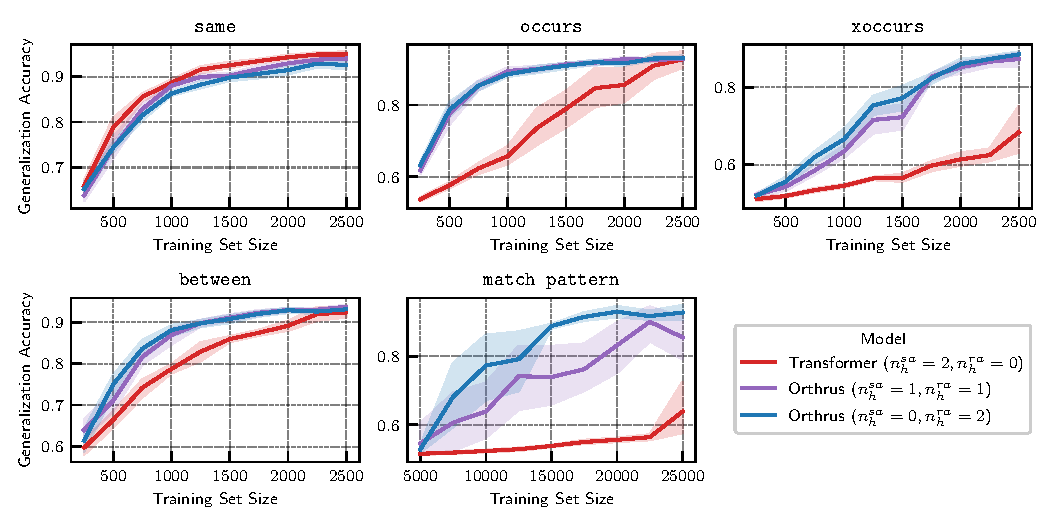
\includegraphics[width=\textwidth]{figs/experiments/relgames/relgames_learning_curves.pdf}
    \caption{Learning curves on the relational games benchmark. Orthrus is more sample-efficient compared to a Transformer with the same total number of heads. Solid lines indicate the mean over 10 trials with different random seeds and the shaded regions indicate bootstrap 95\% confidence intervals.}\label{fig:relgames_learning_curves}
\end{figure}

In this experiment, we use positional symbols as the symbol assignment mechanism since the objects can be identified through their position on the grid. We also impose symmetry on the relations in relational attention, which we find to be a useful inductive bias. Intuitively, this is because the task-relevant relations are symmetric similarity relations across different visual attributes. We provide furhter discussion and present ablations in~\Cref{ssec:appendxi_relgames}.

\aanote[margin,noinline]{legend font size is small, but medium in other figure. make consistent}

\subsection{Improved Symbolic Reasoning in Sequence-to-Sequence tasks: Mathematical Problem Solving}\label{ssec:math}

Next, we evaluate Orthrus on a set of mathematical problem-solving tasks based on the benchmark contributed by~\citet{saxtonAnalyzingMathematicalReasoning2019}. We use this as a proxy for ``symbolic reasoning''. Mathematical problem solving is an interesting test for neural models because it requires more than statistical pattern recognition---it requires inferring laws, axioms, and symbol manipulation rules. The benchmark consists of a suite of mathematical problem solving datasets, with each dataset consisting of a set of question-answer pairs. The tasks range across several modules or topics including solving equations, adding polynomials, expanding polynomials, differentiating functions, predicting the next term in a sequence, etc. For example, a question might be ``\texttt{Expand (5*x - 3) * (2*x + 1).}'' with the target ``\texttt{10 * x ** 2 - x - 3}''.

This is modeled as a sequence-to-sequence model with character-level encoding. We compare Orthrus against a Transformer using matching encoder-decoder architectures. We use 2-Layer models with the total number of heads fixed to $8$ in both the encoder and the decoder. We comapre an encoder-decoder Transformer with $\nhsa = 8$ against two configurations of Orthrus: one with $\nhsa = 4, \nhra = 4$ for the encoder and $\nhsa = 8, \nhra = 0$ for the deocder (config 1) and another with with $\nhsa = 4, \nhra = 4$ for the encoder and $\nhsa = 4, \nhra = 4$ for the decoder (config 2). The number of cross-attention heads is $8$ in all cases. The Orthrus models use position-relative symbols as their symbol assignment mechanism.

\begin{figure}
    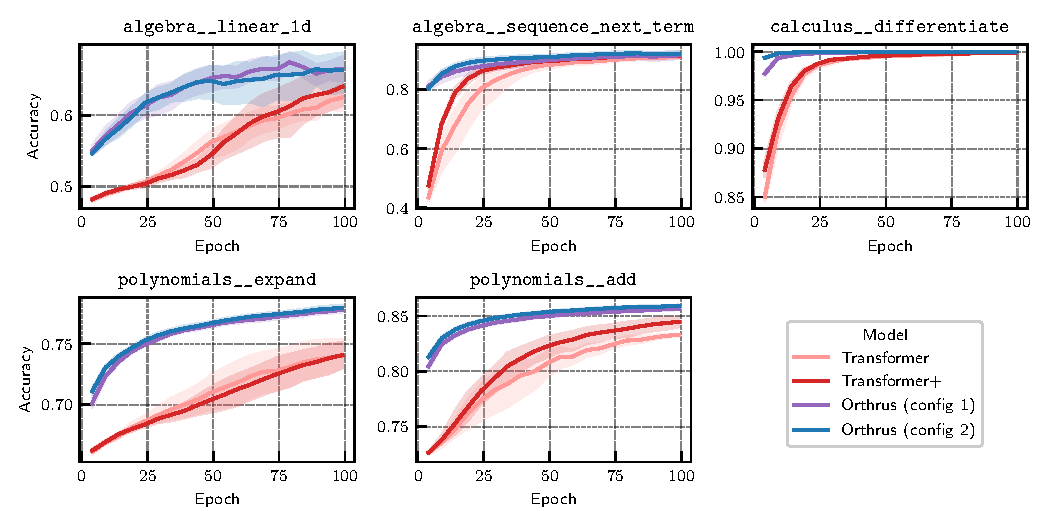
\includegraphics[width=\textwidth]{figs/experiments/math/math_training_curves_interpolation.pdf}
    \caption{Validation accuracy over the course of training on mathematical problem-solving tasks. Orthrus learns faster and reaches higher accuracy. Solid lines indicate mean over 5 trials with different random seeds, and shaded regions indicate 95\% bootstrap confidence intervals.}\label{fig:math_training_curves_interpolation}
\end{figure}

Each model is trained for 100 epochs, and accuracy on a hold-out validation set is tracked over the course of training. For each model and task, we run 5 trials with different random seeds to compute approximate confidence intervals. We find that Orthrus models learn faster and reach higher accuracies compared to a standard Transformer.

\aanote{is Transformer+ discracting? should it be removed or moved to the appendix? it does not make a noticeable difference and reviewers may ask why we don't also do this for the other experiments.}

\subsection{Language Modeling}\label{ssec:tiny_stories}

In this section, we evaluate Orthrus on autoregressive language modeling. Transformer language models are typically built on what is sometimes called a ``decoder-only'' architecture. The model receives a sequence of tokens as input and is trained to causally predict the next token at each position.

We evaluate the language modeling capabilities of Orthrus, as compared to standard Transformers, using the ``Tiny Stories'' dataset of~\citet{eldanTinyStoriesHowSmall2023}. The dataset consists of short stories and is intended as a benchmark for small language models. Again, for each configuration, we fix the total number of attention heads, and compare a Transformer with only standard self-attention heads to Orthrus models with a mix of self-attention and relational attention heads. We compare a Transformer with $\nhsa = 8$ attention heads to two configurations Orthrus, one with $\nhsa = 6, \nhra = 2$ and another with $\nhsa = 4, \nhra = 4$.

\aanote{describe context size, positional encoding, model dimension, batch size, learning rate, etc?}

\begin{figure}[ht]
    % fix d_model and vary n_layers...
    \begin{subfigure}{0.33\textwidth}
        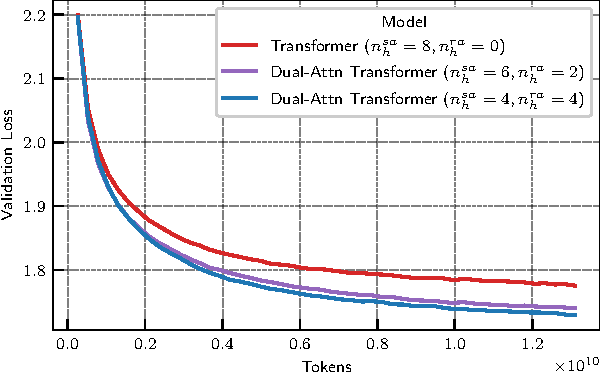
\includegraphics[width=\textwidth]{figs/experiments/tiny_stories/d64L4_symattn_asymra.pdf}
        \caption{4 Layers}
    \end{subfigure}
    \begin{subfigure}{0.33\textwidth}
        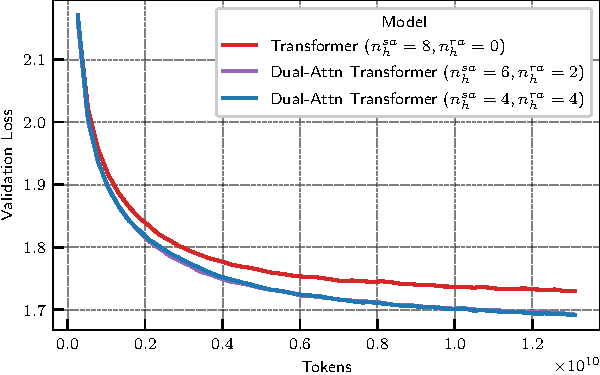
\includegraphics[width=\textwidth]{figs/experiments/tiny_stories/d64L5_symattn_asymra.pdf}
        \caption{5 Layers}
    \end{subfigure}
    \begin{subfigure}{0.33\textwidth}
        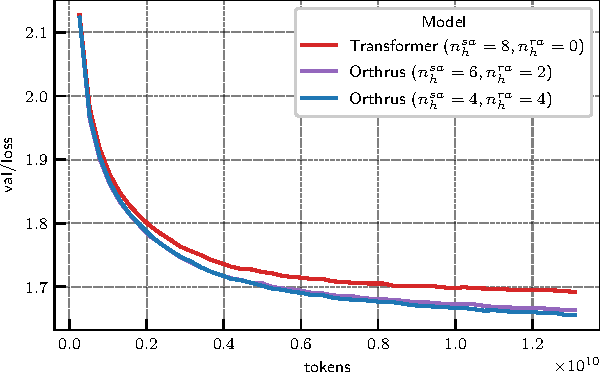
\includegraphics[width=\textwidth]{figs/experiments/tiny_stories/d64L6_symattn_asymra.pdf}
        \caption{6 Layers}
    \end{subfigure}
    \caption{Validation loss curves on a language modeling task. The $x$-axis indicates the number of tokens and the $y$-axis is the validation loss. Orthrus achieves a smaller validation loss for the same total number of attention heads.}\label{fig:tiny_stories_val_loss_curves}
\end{figure}

\Cref{fig:tiny_stories_val_loss_curves} depicts the validation loss over the course of training for each model. We find that Orthrus models with dual head attention achieve lower loss for the same total number of attention heads. We also varied the number of layers, and observed that the trend persists as the number of layers increases. The effect is small but consistent. The two Orthrus configurations behave similarly, with perhaps a very slight advantage to $\nhsa = 4, \nhra = 4$ (the configuration with a balanced composition of head types).

In~\Cref{fig:tiny_stories_val_loss_curves}, the Orthrus models use \textit{symbolic attention} as the symbol assignmnet mechanism and asymmetric relations in relational attention. We find that symbolic attention outperforms position-relative symbols on this language modeling task. In fact, with position-relative symbols, there is no discernable advantage over the Transformer. Symbolic attention may be well-suited to language due to its implementation of a learned differentiable equivalence class mapping, which can perhaps be thought of as a form of syntax. We also find the asymmetric relations in relational attention perform better than symmetric relations. This may be because the relevant relations in language modeling are asymmetric (e.g., asymmetric syntactic or grammatical relations such as noun-verb, subject-object, determiner-noun, etc.). We provide further discussion and present ablations in~\Cref{ssec:appendix_lm}.

We conclude this section by noting that modern large language models are applied to diverse and multi-modal tasks, where different inductive biases will be useful in different contexts. While the language models explored in this section are small, an interesting avenue for future research would be to investigate whether the observed performance benefits scale up to larger models.

\subsection{Multi-modality and potential in vision tasks: ImageNet}\label{ssec:imagenett}
\aanote{how is the acronym ``VAT''? Better than ViAT? VisAT? (Vision Transformer is ViT)}


here, sym\_attn performs worse than transformer, but pos-relative perhaps marginally better?

\section{Discussion}\label{sec:discussion}

\textbf{Summary.} The standard attention mechanism of Transformers provides a versatile mechanism for retrieval of sensory information in any given context, but does not explicitly support retrieval of relational information. In this work, we presented an extension of the Transformer architecture that disentangles and integrates sensory and relational information through a variant of multi-head attention with two distinct types of attention heads: standard self-attention for sensory information and a novel \textit{relational attention} mechanism for relational information. We empirically evaluate this architecture and find that it yields performance improvements across a range of tasks and modalities.

\textbf{Limitations.} The proposed architecture introduces several hyperparameters and possible configurations. Although we carried out ablations on the major configuration choices (e.g., composition of head types, symmetry, symbol assignment mechanism), a more thorough empirical examination would help develop an improved understanding of the behavior of this architecture under different configurations. Such a systematic study may also enable the discovery of further modifications to improve the architecture. We also note that our implementation of the Dual-Attention Transformer lacks the hardware-aware optimizations of standard Transformers~\citep{dao2022flashattention}, making it slower.

\section*{Acknowledgments}
...

\printbibliography


\listoffixmes

\clearpage
\newpage

%%%%%%%%%%%%%%%%%%%%%%%%%%%%%%%%%%%%%%%%%%%%%%%%%%%%%%%%%%%%

\appendix

\section{Function class of disentangled relational cross-attention: a universal approximation result}

Recall that relational cross-attention is a mapping on $\reals^d \times \reals^{n \times d} \to \reals^{d_s}$, where $d$ is the dimensionality of the input objects and $d_s$ is the dimension of the symbols. For convenience, we denote the ``query space'' by $\calX$ and the ``key space'' by $\calY$, though both are the euclidean $\reals^d$ in this setting. Disentangled relational cross-attention takes as input a query $x \in \calX$ and a collection of objects $\y = \ys \in \calY^n$ and computes the following
\begin{align}
  \DisRCA(x, \y) &= \sum_{i=1}^{n} \alpha_i(x; \y) \, r(x, y_i) s_i, \\
  \alpha(x; \y) &= \Softmax\Bigparen{\bigbra{\iprod{\phi_q^{\attn}(x)}{\phi_k^{\attn}(y_i)}}_{i=1}^{n}}, \\
  r(x, y_i) &= \iprod{\phi_q^{\rel}(x)}{\phi_k^{\rel}(y_i)}, \\
  s_i &= \SymbolRetriever\paren{\y; \Slib}_i,
\end{align}
where $\phi_q^{\attn}, \phi_k^{\attn}, \phi_q^{\rel}, \phi_k^{\rel}: \reals^{d} \to \reals^{d_k}$ are the feature maps defining the attention mechanism and the relation, respectively. For our purposes, these are multi-layer perceptrons.

The following result states that Disentangled Relational Cross-Attention can approximate any function of the form: 1) select an object in $\ys$ by an arbitrary query-dependent selection criterion, and 2) compute an arbitrary relation $r: \calX \times \calY \to \reals$ with the selected object. This is formalized below.

To formalize (1), we adopt an abstract and very general formulation of a ``selection criterion'' in terms of family of preference preorders, $\sset{\preceq_x}_x$: for each possible query $x$, the preorder $\preceq_x$ defines a preference over objects in $\calY$ to be selected. Intuitively, ``$y_1 \preceq_x y_2$'' means that $y_2$ is more relevant to the query $x$ than $y_1$.

More precisely, for each query $x \in \calX$, $\preceq_x$ is a complete (for each $y_1, y_2 \in \calY$, either $y_1 \preceq y_2$ or $y_2 \preceq_x y_1$), reflexive ($y \preceq_x y$ for all $y \in \calY$), and transitive ($y_1 \preceq_x y_2$ and $y_2 \preceq_x y_3$ implies $y_1 \preceq_x y_3$) relation. For each $x \in \calX$, $\preceq_x$ induces a preordered space $(\calY, \preceq_x)$. This implicitly defines two additional relations: $\prec_x$ and $\sim_x$. We will write $y_1 \prec_x y_2$ if ``$y_1 \preceq_x y_2$ and not $y_2 \preceq_x y_1$'', and $y_1 \sim y_2$ if ``$y_1 \preceq_x y_2$ and $y_2 \preceq_x y_1$''.

For a collection of objects $\y = \ys \in \calY^n$ and a query $x \in \calX$, the preorder $\preceq_x$ defines a selection function
\begin{equation}\label{eq:def_selection}
  \mathrm{Select}(x, \ys) = \max\paren{\ys, \mathtt{key}=\preceq_x}.
\end{equation}
That is, $\mathrm{Select}(x, \y)$ returns the most relevant element with respect to the query $x$. In particular, it returns $y_i$ when $y_i \succ_x y_j, \ \forall j \neq i$ (and may return an arbitrary element of no unique maximal element exists in $\ys$).

We will assume some regularity conditions on the family of preorders $\sset{\preceq_x}_x$ which essentially stipulate that, 1) nearby elements in $\calY$ have a similar preference with respect to each $x$, and 2) nearby queries in $\calX$ induce similar preference preorders.

\begin{assumption}[Selection criterion is query-continuous and key-continuous]\label{ass:qk_cts}
  The family of preorder relations $\sset{\preceq_x}_{x \in \calX}$ satisfies the following:
  \begin{enumerate}
    \item \textbf{Key-continuity.} ...
    \item \textbf{Query-continuity.} ...
  \end{enumerate}
\end{assumption}

For technical reasons, for \Cref{eq:def_selection} to make sense, we must assume that there exists a unique element to be selected. We formulate this in terms of an assumption on the data distribution of the space $\calX \times \calY^n$. This is a technical assumption, and different forms of such an assumption would be possible (e.g., instead condition on this event).
\begin{assumption}[Selection is unique almost always]\label{ass:select_unique}
  Let $(x, \y) \sim \bbP_{x,\y}$. For each $\epsilon > 0$, there exists $\eta_\epsilon > 0$ such that $\min_{j \neq i} \abs{u_x(y_i) - u_x(y_j)} > \eta_\epsilon$ with probability at least $1 - \epsilon$.
\end{assumption}

\aanote{is $\calX$ and $\calY$ confusing? switch to $\calQ$ and $\calX$ (or $\calK$)?  subscripts in $y$ (e.g., $y_1$) somehow don't look that nice...}

\begin{theorem}[Function class of disentangled RCA]\label{theorem:func_class}
  Let $\calX, \calY$ be compact euclidean spaces. Let $\sset{\preceq_x}_{x \in \calX}$ be an arbitrary family of relevance preorders on $\calY$ which are query-continuous and key-continuous (\Cref{ass:qk_cts}). Let $\mathrm{Select}(x, \ys) = \max(\ys, \mathtt{key}=\preceq_x)$ be the selection function associated with $\sset{\preceq_x}_{x}$. Let $R: \calX \times \calY \to \reals$ be an arbitrary continuous relation function. Suppose $x, \y \sim \bbP_{x, \y}$ and that \Cref{ass:select_unique} holds (i.e., the data distribution is such that there exists a unique most-relevant element). For any $\epsilon > 0$, there exists multi-layer perceptrons $\phi_q^{\attn}, \phi_k^{\attn}, \phi_q^{\rel}, \phi_k^{\rel}$ and a choice of symbols such that,
  \begin{equation*}
    \abs{\DisRCA(x, \ys) - R(x, \mathrm{Select}(x, \ys))} < \epsilon
  \end{equation*}
\end{theorem}

\begin{proof}
  Condition on the event $\calE := \sset{(x, \y) \in \calX \times \calY^n \,\colon\, \min_{j \neq i} \abs{u_x(y_i) - u_x(y_j)} > \eta_\epsilon}$. Let $i^* = \argmax(\ys, \mathtt{key} = \preceq_x) = \argmax(u_x(y_1), \ldots, u_x(y_n))$. By~\citep[Theorem 5.1]{altabaa2024approximation}, for any $\epsilon_1 > 0$, there exists MLPs $\phi_q^{\attn}, \phi_k^{\attn}$ such that $\alpha_{i^*}(x, \y) > 1 - \epsilon_1$ for any $(x, \y) \in \calE$. That is, the attention score is nearly $1$ for the $\preceq_x$-selected element uniformly over inputs in $\calE$.

  Similarly, by~\citep[Theorem 3.1]{altabaa2024approximation}, for any $\epsilon_2 > 0$, there exists MLPs $\phi_q^{\rel}, \phi_k^{\rel}$ such that
  \begin{equation*}
    \abs{R(x, y) - \iprod{\phi_q^{\rel}(x)}{\phi_k^{\rel}(y)}}, \quad \text{Lebesgue almost every } (x, y) \in \calX \times \calY.
  \end{equation*}

  Thus, we have
  \begin{align*}
    &\abs{\DisRCA(x, \ys) - R(x, \mathrm{Select}(x, \ys))} \\
    &= \abs{\sum_{i=1}^{n} \alpha_i(x; \y) \,\iprod{\phi_q^{\rel}(x)}{\phi_k^{\rel}(y_i)} s_i - R(x, y_{i^*})} \\
    &\leq \sum_{i=1}^{n} \abs{\alpha_i(x; \y) \,\iprod{\phi_q^{\rel}(x)}{\phi_k^{\rel}(y_i)} s_i - R(x, y_{i^*})} \\
    &\leq \alpha_{i^*}(x, \y) \abs{\iprod{\phi_q^{\rel}(x)}{\phi_k^{\rel}(y)} s_i - R(x, y_{i^*})} + \sum_{j \neq i^*} \alpha_i(x; \y) \abs{\iprod{\phi_q^{\rel}(x)}{\phi_k^{\rel}(y_i)} s_i - R(x, y_{i^*})}
  \end{align*}
  Let $s_i = 1$ for all $i$, and note that $\max_{x, y} \abs{\iprod{\phi_q^{\rel}(x)}{\phi_k^{\rel}(y)} s_i - R(x, y_{i^*})}$ is finite since $\calX, \calY$ are compact. Then, we have
  \begin{align*}
    &\abs{\DisRCA(x, \ys) - R(x, \mathrm{Select}(x, \ys))} \\
    &\leq (1 - \epsilon_1) \epsilon_2 + \epsilon_1 \max_{x, y, y^*} \abs{\iprod{\phi_q^{\rel}(x)}{\phi_k^{\rel}(y)} - R(x, y^{*})}.
  \end{align*}
  Letting $\epsilon_1, \epsilon_2$ be small enough completes the proof.
\end{proof}

\begin{remark}
  Note that in the construction of $\DisRCA$ in the proof above, we chose symbols as $s_i = 1$. This is because the function class we are approximating in~\Cref{theorem:func_class} only selects an object then computes the relation with it, without encoding the identity of the selected object. Recall that the role of the symbols $(s_1, \ldots, s_n)$ is to encode the identity of each object so that the message from the sender $y_i$ to the receiver $x$ attaches the identity of the sender $s_i$ to the relation $r(x, y_i)$. The ``identity'' of the sender can encode their position in the sequence, their relative position with respect to the receiver, or their syntactic role.
\end{remark}

\section{Code \& Implementation Details}

\aanote{Maybe briefly describe some of the implementational choices made in the public code. Some (pseudo)code for important operations? (e.g., einsum definition of disRCAv2). Describe the options available in public implementation (e.g., choice of symbol assignment mechanism, earlier iterations of RCA and disRCA, choice of activation function in MLP, positional encoding (RoPE, pos-emb), etc.)}

\subsection{Implementation of Disentangled RCA}

\subsection{Implementation of Symbol Assignment Mechanisms}

\subsection{Implementation of Encoder and Decoder Blocks}

\subsection{Other versions and iterations of RCA}

\subsection{Miscellaneous: MLP block, Positional Encoding, Normalization, etc.}

\section{Comparison to~\citet{altabaa2024abstractors}}

\aanote{compare RCA to disRCA, discuss motivation for choices made, discuss limitations of the Abstractor framework that are addressed herer, etc.}

\end{document}